\documentclass[pdflatex,sn-nature]{sn-jnl}
\usepackage{graphicx,booktabs,array,amsmath,amssymb,xurl,placeins}
\geometry{reset,a4paper,twoside,bindingoffset=6mm,margin=23mm}
\hypersetup{bookmarksdepth=2}
\emergencystretch=2em
\raggedbottom
\setlength{\bibsep}{0pt}

% begin numbers.tex
\newcommand{\PopTwenty}{1.665}
\newcommand{\BuiltTwenty}{197.5}
\newcommand{\PopPctTwenty}{7.40}
\newcommand{\PopThirty}{3.020}
\newcommand{\BuiltThirty}{325.6}
\newcommand{\PopPctThirty}{13.42}
\newcommand{\PopForty}{4.891}
\newcommand{\BuiltForty}{464.6}
\newcommand{\PopPctForty}{21.74}
\newcommand{\PopTotal}{22.501}
\newcommand{\BuiltTotal}{1253.6}
\newcommand{\UniformOneMin}{4.763}
\newcommand{\UniformBiasMin}{57.7}
\newcommand{\UniformOneMax}{4.770}
\newcommand{\UniformBiasMax}{57.9}
\newcommand{\GHSLJointPct}{13.37}
\newcommand{\GHSLJointCommon}{2.989}
\newcommand{\WPJointPct}{23.20}
\newcommand{\WPJointCommon}{5.186}
\newcommand{\EpochOldPct}{20.86}
\newcommand{\EpochOldCommon}{4.664}
\newcommand{\EpochNewPct}{20.28}
\newcommand{\EpochNewCommon}{4.534}
\newcommand{\JointExcluded}{142.9}
\newcommand{\SampleTwentyEight}{3.051}
\newcommand{\SampleFiftySix}{3.232}
\newcommand{\SampleOneTwelve}{3.369}
\newcommand{\SampleTwoTwentyFour}{3.301}
\newcommand{\DWRTotal}{598098}
\newcommand{\DWRUnsupported}{1710}
\newcommand{\DWRSupportPct}{99.71}
\newcommand{\DWRUniformMin}{9022}
\newcommand{\DWRUniformMax}{9556}

% end numbers.tex


% begin round2_numbers.tex
\newcommand{\InteriorPopulationMin}{99.27}
\newcommand{\InteriorPopulationMax}{99.49}
\newcommand{\InteriorBiasMin}{58.24}
\newcommand{\InteriorBiasMax}{58.56}
\newcommand{\InteriorErrorMin}{98.55}
\newcommand{\InteriorErrorMax}{98.87}

% end round2_numbers.tex


% begin cross_numbers.tex
\newcommand{\CrossGHLow}{51.3}
\newcommand{\CrossGHHigh}{55.6}
\newcommand{\CrossWPLow}{8.6}
\newcommand{\CrossWPHigh}{9.1}

% end cross_numbers.tex

\begin{document}
\title[Spatial allocation and InSAR support]{Quantifying how spatial allocation and sampling alter population-weighted InSAR support summaries}
\author[1]{\fnm{Zixuan} \sur{Liu}}
\author*[2,3]{\fnm{Wei} \sur{Xiong}}\email{xw@mail.hbut.edu.cn}
\affil[1]{\orgname{Detroit Green Technology Institute, Hubei University of Technology}, \orgaddress{\city{Wuhan}, \postcode{430068}, \country{China}}}
\affil[2]{\orgname{School of Electrical and Electronic Engineering, Hubei University of Technology}, \orgaddress{\city{Wuhan}, \postcode{430068}, \country{China}}}
\affil[3]{\orgname{Department of Computer Science and Engineering, University of South Carolina}, \orgaddress{\city{Columbia}, \postcode{29201}, \state{SC}, \country{USA}}}
\abstract{Population-weighted InSAR support summaries depend on the alignment of population and observations within reporting units. We quantify this interaction with matched-input allocation comparisons, controlled missingness and population-model/sampling sensitivities. In a fixed Chao Phraya footprint, native GHSL allocation gives a mean area--pair support deficit of 3.020 million allocation units. Uniform allocation of the same population within 1-km cells raises the deficit by 57.7--57.9\% (+7.75--7.78 percentage points of total allocation). Within-cell covariance explains this effect, which persists after boundary cells are excluded. Crossing GHSL and WorldPop with two pair selections preserves its direction while changing its magnitude. A connected LiCSBAS experiment separates sampled support from final quality; the final-mask allocation shift is only 0.108--0.117 percentage points. Further tests use actual Census blocks, contiguous holes, training-only quality curves, spatial/date dependence, municipal eligibility and two California regions. Small regional effects, unidentified allocation under contiguous holes and mixed external GNSS consistency constrain generalization. The results support mass-preserving accounting with explicit allocation and coverage limits. The deficit averages model allocation over area and pairs; it does not establish deformation in missing locations.}
\keywords{InSAR, population allocation, observation support, coherence, spatial scale, reproducibility}
\maketitle
% The sn-jnl class globally disables top floats while formatting the title.
% Restore ordinary in-text float placement after the title page is complete.
\makeatletter\global\@topnum=5\makeatother
\raggedright

\section{Introduction}
Interferometric synthetic aperture radar (InSAR) measures ground displacement at locations supported by the acquisition geometry, scattering properties and processing network. Persistent-scatterer, small-baseline and distributed-scatterer approaches explicitly address this selective measurement process \citep{ferretti2001ps,berardino2002sbas,ferretti2011squeeSAR}. LiCSBAS and MintPy provide established diagnostics for unwrapped coverage, coherence, temporal connectivity, residuals and uncertainty \citep{morishita2020licsbas,yunjun2019mintpy}. A downstream population overlay introduces a further question: how does the spatial placement of population within a reporting unit interact with the support represented by a particular diagnostic or product?

Published exposure studies make different, often explicit choices. Blackwell et al. combined multiple radar datasets with GNSS and estimated California community exposure under a uniform-within-community population assumption \citep{blackwell2020california}. The Mexico-wide assessment applied temporal-coherence screening, compared velocities with GPS and reported population and households in detected subsiding urban localities \citep{fernandeztorres2024mexico}. Ao et al. reported urban population shares above InSAR-rate thresholds \citep{ao2024national}. Ohenhen et al. mapped 28 US cities at about 28-m resolution, checked rates against 154 GNSS stations and assigned census-block population to rate classes using each block's median InSAR-pixel rate \citep{ohenhen2025uscities}. Recent work extends exposure analysis to nationwide population, building and infrastructure inventories, building-level diagnostic risk, and coastal population-weighted relative sea-level rise with integrated vertical-land-motion uncertainty \citep{xiong2026nationwide,yang2026buildingrisk,oelsmann2026coastal}. Those studies estimate different endpoints using broader inventories or calibrated deformation products; they motivate careful separation of observed support, population allocation and uncertainty, but do not supply independent validation for our Bangkok LOS field. Murray et al. explicitly noted that motion between buildings may remain undetected and require additional observations \citep{murray2025hawaii}. These studies establish relevant applications and careful measurement practice; their reporting units and target quantities differ. They do not establish that users generally misinterpret missing support. Published Bangkok leveling and CORS comparisons provide further examples of geodetic validation, with spatial, temporal and station-specific qualifications detailed in Supplementary S8 \citep{luachapichatikul2020bangkok,pumpuang2024bangkapi,aieorattanawadee2022bangkok}.

Population disaggregation and areal interpolation also have an established methodological basis. Eicher and Brewer evaluated alternative dasymetric mapping procedures, while Mennis combined areal weighting and ancillary land-cover information to estimate finer population surfaces \citep{eicher2001dasymetric,mennis2003population}. A finer allocation can preserve the selected model's spatial structure without establishing household-level accuracy. Our question concerns a specific operation in downstream reporting: replacing the joint population--support distribution inside a coarse unit by its separate averages. The resulting difference depends on their spatial covariance, whose magnitude and direction must be assessed for the actual inputs. This is a testable allocation effect even when the upstream product correctly documents its quality.

We ask three questions. First, with the geographic domain, support field and population total fixed, how much do center sampling, uniform coarse allocation and native-model allocation change the reported summary, and what explains the difference? Second, how does that effect vary with grid scale and origin, introduced missingness, interferogram selection and population model? Third, how does sampled support relate to one specified processing chain's final quality and to a second product's published observation footprint? We address these questions through matched-input comparisons, controlled missingness, expanded sampling, alternative population models, a connected LiCSBAS experiment and a Fresno coverage example. The contribution is a matched-input evaluation of the size, direction and population-model dependence of aggregation effects, together with a protocol for preserving the population--support cross moment. The sequence of experiments establishes the effect, explains its mechanism and tests its applicability across inputs and support definitions.

\section{Materials and methods}
\subsection{Separate the geographic domain, support field and allocation model}
We distinguish three objects: the geographic domain $D$ (area of interest, AOI), a support field $s(x)\in[0,1]$, and a nonnegative exposure density $\rho(x)$. Our primary Chao Phraya domain is the native Global Human Settlement Layer (GHSL) pixels whose centers lie in the frozen finite footprint of 18,077 archived VLM cells. It includes 1,807,700 GHSL 3-arc-second pixels and does not condition on a velocity threshold. This explicit pixel-defined boundary is held fixed in all primary allocation experiments. Because its footprint is inherited from finite source-product cells, this design does not assess locations outside that original footprint or establish complete coverage of the geographical delta.

The archived VLM GeoTIFF matches the Chao Phraya file in the global-delta dataset accompanying Ohenhen et al. \citep{ohenhen2026deltas,ohenhen2025deltadata}. That study used WabInSAR. Our LiCSAR quality sample is a different processing chain and cannot be interpreted as the validity mask of the WabInSAR product. Moreover, the public GeoTIFF lacks an explicit stored-unit tag establishing the archived factor-of-ten conversion. We therefore retain the inherited strong-deformation selection only as a clearly labeled supplementary sensitivity. Neither that conversion nor a cross-product quality proxy determines the primary geographic population denominator.

For pair $j$, let $M_j(x)$ be one when unwrapped phase is finite, passes its raster validity mask and is nonzero, and, for the joint screens, the associated byte coherence divided by 255 is at least $q$. The unwrapped zero rule is product-specific \citep{licsarproducts}. We evaluate $q=0.2,0.3,0.4$ and unwrapped validity alone. Source-grid boundaries and the actual GDAL affine transforms, including point registration, are used independently for coherence and unwrapped products. We split at both sets of boundaries, intersect the binary masks first, and then integrate. Multiplying separately averaged fractional masks would not give their spatial intersection.

For GHSL pixel $p$ with area $A_p$, the reported support is
\begin{equation}
s_p=\frac{1}{N A_p}\sum_{j=1}^{N}\int_p M_j(x)\,\mathrm{d}A.
\label{eq:support}
\end{equation}
Thus $s_p$ is mean area--pair support at the exposure grid. It is distinct from the area whose individual locations pass a fixed number of pairs, from a binary majority classification at a cell center, and from final inversion validity. We assume each GHSL pixel's population or built-surface total is uniform within that pixel when integrating its intersections. Spherical rectangular areas use longitude and sine-latitude boundaries.

\subsection{Continuous summaries and what they do not estimate}
With nonnegative allocated exposure $E_p$, define supported allocation $S_E=\sum_p E_p s_p$, mean support deficit $U_E=\sum_p E_p(1-s_p)$, and total $T_E=\sum_p E_p$. By construction, $S_E+U_E=T_E$. Population-valued $U_E$ is an average unsupported allocation over the selected pairs. For example, a pixel assigned 100 people and mean support 0.8 contributes 20 population-allocation units to $U_E$. Those units express a weighted average over area and pairs; they do not identify 20 particular residents. As an allocation example, two equal-area fine pixels with populations 90 and 10 and supports 1 and 0 have a native deficit of 10. Spreading the same total uniformly across their combined area gives 50. Reversing the support pattern gives a native deficit of 90 and the same uniform estimate of 50. These constructed examples explain both the units and possible error directions. It is not the number of unique people never observed during the entire period. Neither population-valued nor built-surface-valued $U_E$ identifies confirmed deformation, vulnerability, loss or damage.

The weighted support distribution is
\begin{equation}
F_E(t)=\frac{\sum_p E_p\,\mathbf{1}(s_p<t)}{T_E},\qquad
\int_0^1 F_E(t)\,\mathrm{d}t=\frac{U_E}{T_E}.
\end{equation}
We show the full distribution rather than selecting a single majority cutoff. The integral identity concerns the empirical step distribution; its exact numerical check uses the sorted support values, not a trapezoidal approximation to the 101-point display curve. These are accounting identities, not new statistical theorems.

\subsection{Matched-target allocation and grid experiments}
The center, area-weighted and ancillary-weighted rules represent distinct choices within established areal-interpolation practice \citep{eicher2001dasymetric,mennis2003population}. Supplementary S10 states their information requirements and which comparisons are actually performed. Native GHSL allocation is the common model reference for these tests; comparisons with deformation imputation or multi-sensor retrieval would require a different target and additional observations.

We conservatively transfer extensive first and cross moments to a 50-m UTM integration grid (zone 47N), then repartition them into 250-, 500-, 1,000- and 2,000-m cells. Each size has four origins formed by zero and half-cell shifts in each axis. Included-domain area is retained in partial boundary cells; population is not extrapolated into the omitted area. The tested production transfers preserve input totals to numerical precision. A separately recomputed 25-m integration diagnoses approximation sensitivity, including its measured small reprojection drift (Supplementary Information).

Within cell $c$, let $P_c=\int_c\rho\,\mathrm{d}A$, $H_c=\int_c\rho s\,\mathrm{d}A$, $A_c=\int_c\mathrm{d}A$ and $Q_c=\int_c s\,\mathrm{d}A$. Native-model reference deficit is $P_c-H_c$, while uniform allocation gives $P_c(1-Q_c/A_c)$. Their difference is
\begin{equation}
U_{\rm uniform}-U_{\rm native}
=\sum_c\left(H_c-\frac{P_c Q_c}{A_c}\right)
=\sum_c A_c\operatorname{Cov}_{A,c}(\rho,s).
\label{eq:covariance}
\end{equation}
Preserving $H_c$ avoids replacing the native reference with the product of separately averaged population and support fields. The center method applies support from the fine pixel containing each coarse center; centers outside the fixed domain receive zero support. Its boundary behavior is therefore explicit. We report signed aggregate differences, errors relative to the fixed AOI total, and cell-level absolute errors. The native GHSL reference is a controlled allocation model, not observed household truth. To separate interior allocation effects from boundary handling, we additionally repeat the primary comparison on coarse rectangles wholly contained in the pixel-defined domain. The domain boundary is formed from the native GHSL mask, densified at native-pixel spacing and transformed to UTM before the containment test. Interior and boundary subsets retain their own population and reference-deficit denominators; full-domain results remain the primary comparison.

\subsection{Artificial masking with known reference quantities}
A fixed Bangkok rectangle (100.35--100.75$^\circ$ E, 13.55--13.95$^\circ$ N) supplies the population and built-surface fields for controlled masking. This rectangular experiment is separate from the VLM-footprint domain. We remove 10\%, 30\% or 50\% of fine pixels using random scores, spatially smoothed random scores, and scores positively or negatively associated with log population density. We fix the seed and run 100 repetitions per combination. All scenarios, including opposite bias directions, are retained.

Methods use identical introduced masks and coarse-cell population totals. We compare uniform-area allocation, center sampling and allocation proportional to fine built area, with an area fallback where built area is zero. Grids contain 5, 10 or 20 native pixels with two origins; these angular grids are not described as exact metric cells. We evaluate against the known removed allocation $U_{\rm ref}$. Percentile ranges describe variation over the introduced masks, conditional on the fixed models. They are not confidence intervals for real population or InSAR accuracy. Built weighting is not independent validation because GHSL population already uses built-environment information.

We also construct three explicit synthetic hazard fields: positive density association, negative association and an independent spatial field. Rates are assigned either $-10$ or $0$ mm yr$^{-1}$ solely to define known threshold membership. For observed threshold allocation $T_{\rm obs}$ and unknown allocation $U$, the nonparametric identification interval is $[T_{\rm obs},T_{\rm obs}+U]$. Checking that synthetic truth lies inside this interval verifies the accounting bound; it does not validate a physical prediction or establish 95\% coverage.

\subsection{Sampling, population products and land cover}
The legacy sample has 28 pairs from 2016--2022. We evaluate year omissions, start-date quarters and temporal-baseline groups. A larger pool contains eight pairs per year--quarter stratum, totaling 224. Selection uses dates and short/long baseline classes before expanded support outcomes are computed. Before outcome extraction, adjacent ranks in even quarters were swapped to improve balance in the smallest nested sample; both rank plans and the amendment are preserved. Available baseline composition is reported explicitly. Nested ranks produce 28, 56, 112 and 224 pairs. An additional 100 draws without replacement per sample size characterize sampling variation within this fixed pool. They do not account for unknown interferograms outside the pool, nor estimate independent-observation confidence bounds.

We compare GHSL R2023A epoch-2020 population at 3 arcsec with WorldPop's Thailand 2020 unconstrained UN-adjusted population-count product at 3 arcsec \citep{pesaresi2024ghsl,worldpop2020}. Source counts are transferred by spherical source-area fractions, not by interpolation of density values as if they were counts. Native totals, jointly valid coverage and common-total normalized results are all reported. GHSL 2015/2020 epoch comparisons hold resolution at 30 arcsec. Neither population product is local census truth, and epoch differences combine demographic and model effects.

\paragraph{Crossed aggregation sensitivity.} To test the aggregation effect directly across inputs, we cross GHSL and WorldPop 2020 allocations with the legacy 28-pair and expanded 224-pair support fields at $q=0.3$. All four combinations use the same two-model common-valid domain and the same total population, set to the GHSL total on that domain. The domain is fixed before comparing aggregation outputs. Each combination compares native-model and uniform allocation within 1-km cells at four origins, using conserved area, supported area, population and population--support cross moments. We report differences relative to the native-model deficit and to the common total. A 25-m integration diagnostic checks the production 50-m transfer. Pair selection and composition change with pair number; the experiment does not isolate sample size alone. Supplementary S12 retains all 16 model--sample--origin cases.

ESA WorldCover 2021 v200 provides native 10-m land classes \citep{worldcover2021}. We calculate their fractional areas inside each GHSL pixel and allocate that pixel's population uniformly across those fractions. The resulting class summaries describe model allocation; for example, an allocation to tree-cover fractions is not evidence that particular residents occupy trees. The 2021 land-cover epoch also differs from the population epoch and the multi-year radar sample.

\subsection{Computational assistance}
An OpenAI Codex assistant was used during this revision to assist experimental code development, numerical checks, figure generation and manuscript drafting. Reported numerical outputs were produced by executing the retained scripts against the documented inputs. This assistance does not supply independent observations or physical validation.

\subsection{Matched processing and a second published-support case}

% begin matched_methods.tex
We define a separate Bangkok urban--periurban rectangle (100.35--100.65$^\circ$ E, 13.65--14.05$^\circ$ N) before examining processing outcomes. All 437 catalogue pairs with both dates in 2019--2020 and temporal baseline at most 96 days are retrieved and checked. This date graph contains 104 acquisitions and is connected. Native unwrapped phase and byte coherence are aligned by nearest sampling, using each source's actual GDAL transform, onto the first unwrapped raster's approximately $0.001^\circ$ grid. LiCSBAS2 steps 11--16 provide quality rejection, loop closure, small-baseline inversion, velocity spread, multi-index masking and filtering \citep{morishita2020licsbas,licsbas2}. We retain upstream scientific routines and fixed C-band defaults; automatic relaxation of masking thresholds is disabled. Supplementary S7 records the exact version and parameters.

Before reading pixel quality, 44 pair edges are randomly selected for holdout while preserving global acquisition-date connectivity. The other 393 pairs are processed separately through the same workflow. Held-out phase differences are converted to relative line-of-sight (LOS) displacement and referenced to the training solution's reference pixel. Predicted differences come from the unfiltered training cumulative displacements at those two dates. On observations evaluable by all methods, we also compare predictions from the training linear velocity and from zero relative displacement. Missing training dates or invalid held-out phase at the training reference are recorded as exclusions. Predictive strata use training-pair support and the training mask, excluding held-out coherence from their definition. All held-out dates remain represented in training; this tests edge reconstruction rather than forecasting new acquisition dates. Pairs share acquisitions and date-dependent atmospheric phase, so we report descriptive residuals without an independent-replicate confidence interval. No GNSS calibration, vertical decomposition or recovery of permanently absent observations is claimed.

We separately compare legacy 28-pair support and matched-stack support with the full-stack quality mask, reporting pixel- and population-weighted confusion counts, support-bin validity, velocity spread and inversion residuals. Native GHSL counts are transferred by source-area fractions to the processing grid. Mask association is partly built into the algorithm because coherence contributes to its quality criteria; the edge holdout adds a distinct internal predictive check. The legacy comparison additionally differs in acquisition period (2016--2022 versus 2019--2020); the matched input diagnostic provides a within-period comparison. This experiment evaluates a specified LiCSAR/LiCSBAS chain and does not test the validity of the WabInSAR source raster.

% end matched_methods.tex


For the independent geometry case, we select a fixed Fresno rectangle (119.9--119.7$^\circ$ W, 36.6--36.85$^\circ$ N) before inspecting its support results. The California Department of Water Resources (DWR) 2026Q1 service supplies actual polygons representing its 100-m measurement cells \citep{dwr2026,dwrdocumentation}. We download all 38,738 intersecting cells, verify their geometry, clip them to the AOI and compute their nonduplicated union within native GHSL pixels. We do not assign the full population of a source pixel separately to each measurement point. The same metric scale/origin comparison is repeated in UTM zone 11N, and artificial masking is repeated within the published observed footprint. This case tests transfer of support accounting to a final published observation footprint; its polygon layer alone provides no per-cell velocity or uncertainty. We do not infer motion in its gaps. Its 2015--2026 observation record and 2020 population also have an explicit temporal mismatch.


% begin additional_methods.tex
\subsection{Additional robustness and transfer tests}
We extend the controlled comparison to actual irregular 2020 Census blocks in Fresno. Complete-block GHSL allocations are normalized to the official P1 total before restriction to cells with known DWR annual rates for 1 October 2020--1 October 2021. Random removals and one or four contiguous holes remove 10, 30 or 50\% of known-rate cells, with 30 repetitions and fixed thresholds of $-3$, $-5$ and $-10$ mm yr$^{-1}$. Native observed-allocation prevalence, observed-area prevalence and a published pixel-centre unit-median-rate rule use identical masks. Blocks without the information required by a rule remain undefined. We report method-specific unestimated allocation, error on the common-computable domain and worst-case bounds on the whole originally known domain (Supplementary S25).

To address dependence, we perform exploratory five-band spatial holdouts for recalibrating released population grids against ACS, with west--east and south--north designs and 0-, 1- and 3-km exclusion buffers. The total multiplier uses training groups only; this is not cross-validation of the original population-model training. We also remove all sampled pairs incident to each acquisition date from the 224-pair support pool and recompute equal-pair/equal-quarter summaries, without re-inverting velocities (S26). For the connected processing stack, 18 rules based only on training-mask, coherence, residual or velocity-standard-deviation information are applied to the fixed training inversion. Full-domain coverage and internal displacement residuals across all 44 excluded edges are reported jointly; no threshold is chosen from held-out error (S27).

Two further rectangles, Los Angeles and Davis--Sacramento, are fixed before outcome inspection and evaluated across three coherence cutoffs, four metric scales and four origins using archived ARIA California LOS/coherence products \citep{sangha2026california,sangha2026data} (S28). An independent municipal land-use classification supplies residential eligibility in Fresno, with strict and broader mixed-use rules and an explicit unmapped category \citep{fresno2026landuse} (S29). Finally, archived NGL GNSS LOS estimates are compared with the external California product over its documented track periods. Provider reference sites and one location-selected local frame-control site per region are excluded from every validation metric. The two spatial-frame choices and all three sampling radii are retained. Archived linear GNSS fits differ from the InSAR temporal model; this comparison is neither a fresh daily-GNSS refit nor validation of our Bangkok inversion (S30).

% end additional_methods.tex


\section{Results}
\subsection{Spatial support and allocation have different weighted distributions}
The fixed Chao Phraya footprint contains \PopTotal{} million GHSL population units and \BuiltTotal{} km$^2$ of built surface. At $q=0.3$, native allocation gives $U_E=\PopThirty{}$ million population units (\PopPctThirty{}\%) and \BuiltThirty{} km$^2$ of built surface. Population is concentrated in relatively well-supported portions of the footprint (Fig.~\ref{fig:spatial}). Consequently, area-, built-surface- and population-weighted support distributions differ (Fig.~\ref{fig:curves}).

\begin{figure}[htbp]\centering
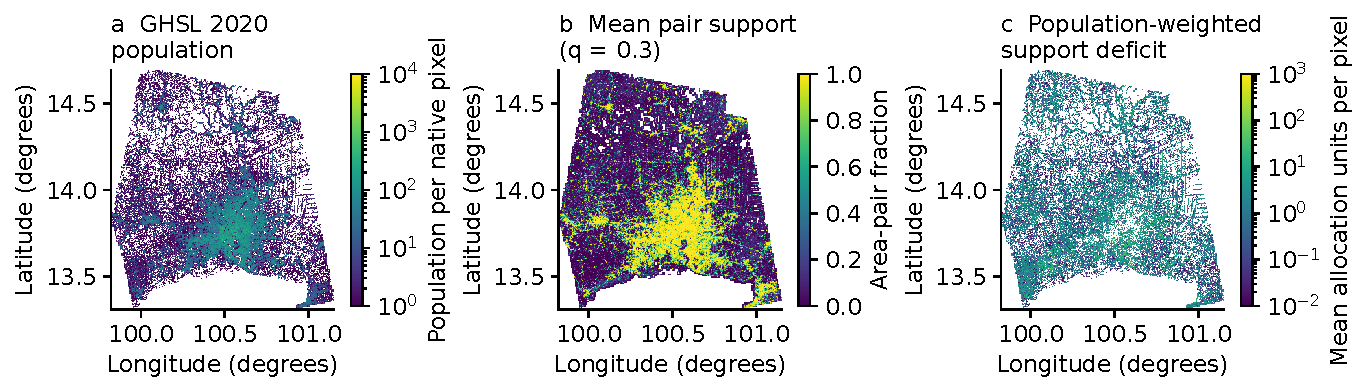
\includegraphics[width=\linewidth]{figures/F1_chao_spatial.pdf}
\refstepcounter{figure}\label{fig:spatial}
\end{figure}
\begin{table}[htbp]\centering
\refstepcounter{table}\label{tab:baseline}

% begin baseline_table.tex
\begin{tabular}{lrrrr}\toprule
Support rule & Population & Pop. (\%) & Built surface & Area (\%)\\\midrule
Valid unwrapped & 0.268 & 1.19 & 31.9 & 17.89 \\
Joint, $q=0.2$ & 1.665 & 7.40 & 197.5 & 57.44 \\
Joint, $q=0.3$ & 3.020 & 13.42 & 325.6 & 68.77 \\
Joint, $q=0.4$ & 4.891 & 21.74 & 464.6 & 76.83 \\
\bottomrule\end{tabular}

% end baseline_table.tex

\end{table}

Unwrapped validity alone and the coherence-screened quantities are substantially different (Table~\ref{tab:baseline}). Raising $q$ from 0.2 to 0.4 changes the mean population deficit from \PopTwenty{} to \PopForty{} million. This range is a definition sensitivity, not a confidence interval. The weighted support curves retain information lost by applying one majority threshold to every coarse cell.

\begin{figure}[htbp]\centering
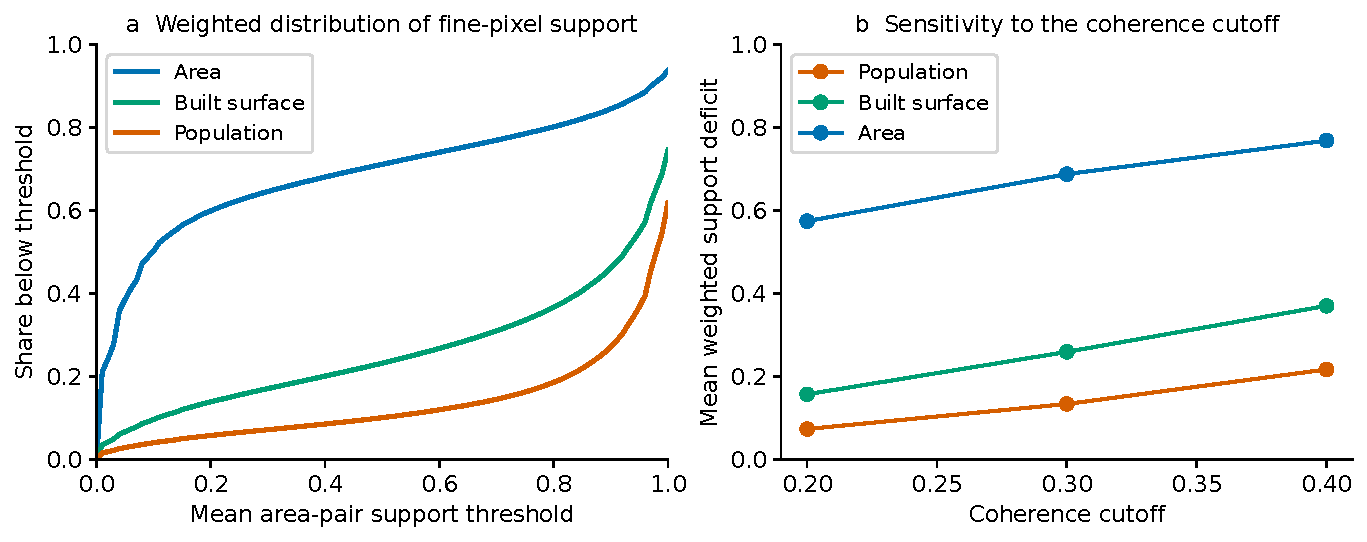
\includegraphics[width=\linewidth]{figures/F2_support_curves.pdf}
\refstepcounter{figure}\label{fig:curves}
\end{figure}

\subsection{Coarse uniform allocation changes the target materially}
With support, native population and AOI total held fixed, uniform allocation within 1-km cells yields \UniformOneMin{}--\UniformOneMax{} million mean population units in deficit, compared with the native-model reference of \PopThirty{} million. This is \UniformBiasMin{}--\UniformBiasMax{}\% higher across the four origins. Aggregate error grows across the examined 250--2,000-m scales (Fig.~\ref{fig:scale}). The center approximation also changes with scale and origin; its variability cannot be interpreted as a measurement uncertainty distribution.

The signed discrepancy equals the integrated population--support covariance in Eq.~\ref{eq:covariance}. Positive aggregate covariance in this case means that uniform redistribution moves some population away from better-supported fine locations. Individual cells can have either sign, as the local error plot shows. Increasing the number of output cells is therefore not the sole explanation: the relative placement of population and support within those cells is decisive. Projection to a 25-m rather than 50-m integration grid changes the 1-km uniform population estimate by at most 0.00024 percentage points of the AOI total, far below the allocation differences being compared. A separate pixel-centre grouping diagnostic across 250--2,000-m squares reproduces the covariance identity to numerical precision and satisfies its Cauchy--Schwarz bound; these scale-sensitivity values are not pooled with the direct-geometry estimates (Supplementary S15).

The 1-km effect persists when all boundary-crossing cells are excluded. Across four origins, the complete interior cells contain \InteriorPopulationMin{}--\InteriorPopulationMax{}\% of domain population, and uniform allocation exceeds their own native-model deficit by \InteriorBiasMin{}--\InteriorBiasMax{}\%. Interior cells account for \InteriorErrorMin{}--\InteriorErrorMax{}\% of the full-domain signed uniform-allocation difference. Thus boundary treatment does not explain the primary allocation effect. Supplementary S11 separates complete, partial and outside-center cells and reports both methods under each origin.


\begin{figure}[htbp]\centering
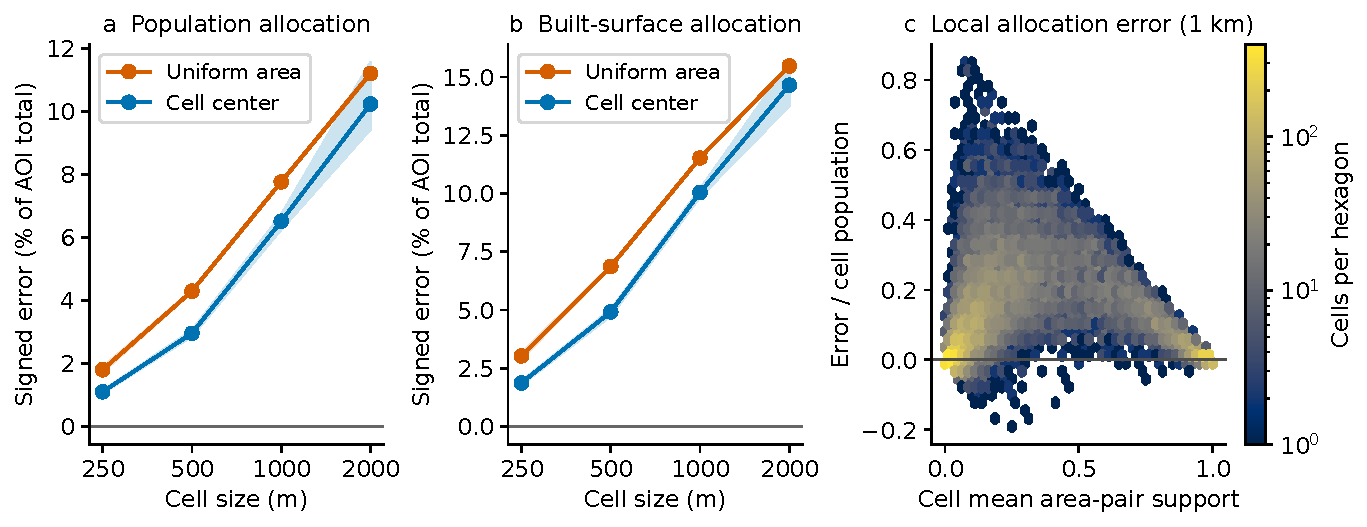
\includegraphics[width=\linewidth]{figures/F3_allocation_scale.pdf}
\refstepcounter{figure}\label{fig:scale}
\end{figure}

\subsection{Controlled missingness identifies both useful and failing cases}
For random and spatial masks unrelated to density, aggregate mean bias is small across repetitions, while the center method has larger sample-to-sample variation. Density-associated masking changes the sign and size of the error (Fig.~\ref{fig:masking}). At 30\% removal and 10-pixel cells with zero origin, uniform allocation underestimates the known removed population by 14.17\% when high-density locations are preferentially removed and overestimates it by 120.35\% when low-density locations are preferentially removed. Very large relative errors at low removed-population denominators are accompanied by errors normalized to the entire test population and are not presented without that context.

Built-area weights reduce error in these GHSL-based scenarios but retain nonzero errors and shared-input dependence. The synthetic hazard experiments additionally show that support deficit alone does not identify threshold-exposed population: the unknown allocation can contain very different hazard shares under the three constructed velocity fields. The conservative identification interval contains the known truth by construction; its width expresses missing information rather than recovered motion. Fresno masking outputs repeat the same protocol and are supplied in the Supplementary Information.

We further compared unit-median assignment with within-unit observed-population prevalence under controlled masks on the actual fitted LOS field. Across four mask mechanisms, 100 repeats and four fixed origins, neither estimator dominates: median assignment is closer under preferential removal of low-spread pixels, whereas prevalence has smaller mean signed error under random and clustered masks. Under preferential removal of high-spread pixels all three methods underestimate the known class allocation. Because the LOS field was artificially masked only where it was originally valid, this benchmark evaluates estimator behavior under specified missingness and does not resolve genuinely unsupported locations (Supplementary S22).

For the actual LiCSBAS final mask, a worst-case finite-domain calculation bounds the share of allocation in each LOS threshold class without assigning a physical rate to unsupported pixels. Unsupported allocation accounts for 0.2944 percentage points of the fixed domain, so the identification interval has that width at each of the $-2$, $-5$ and $-10$ mm yr$^{-1}$ thresholds. This finite bound is small in population-share terms but leaves the motion in unsupported locations unknown (Supplementary S21). We also show how a user-selected aggregate-error tolerance can be compared with the analytic scale/origin bound; coarse scales often remain inconclusive even where the net observed difference is smaller (Supplementary S23).


\begin{figure}[htbp]\centering
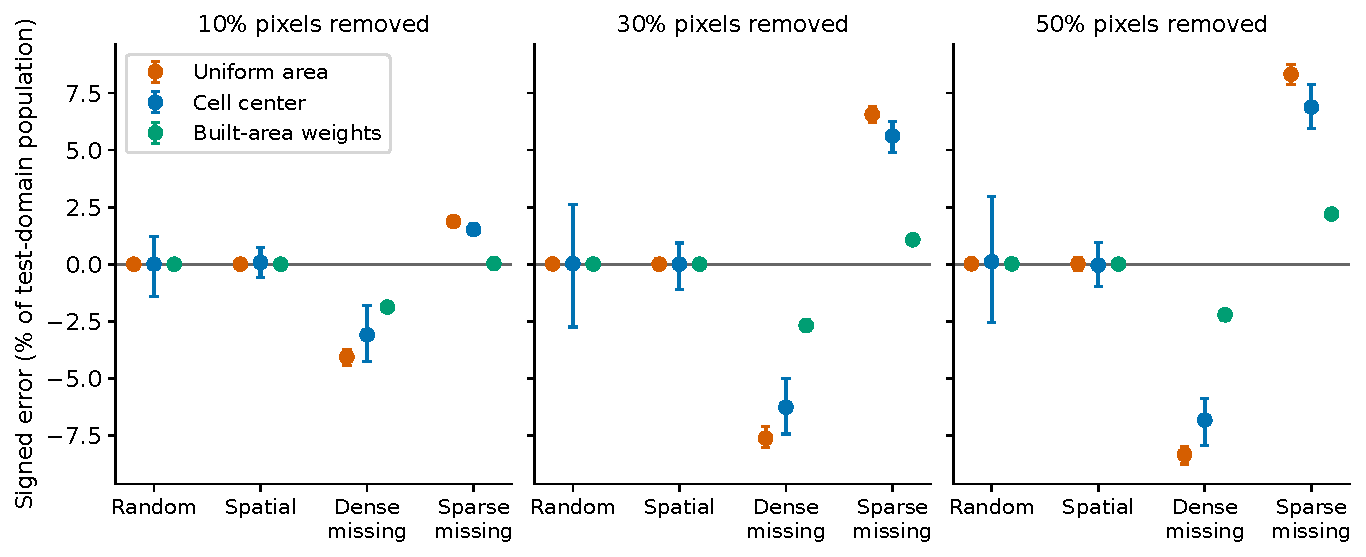
\includegraphics[width=\linewidth]{figures/F4_masking.pdf}
\refstepcounter{figure}\label{fig:masking}
\end{figure}

\subsection{Sampling and population choice remain consequential}
The legacy 28-pair date graph contains 54 dates, 26 components and no independent cycles. It cannot stand in for a complete time-series inversion network. The 224-pair sampling graph is also not fully connected: it has 225 dates and 29 components. In contrast, the 2016--2022 catalogue graph has 288 dates and one component. Catalogue-level connectivity does not establish pixel-level validity.

The nested 28-, 56-, 112- and 224-pair means give population deficits of \SampleTwentyEight{}, \SampleFiftySix{}, \SampleOneTwelve{} and \SampleTwoTwentyFour{} million, respectively (Supplementary Fig.~S1). The nested 28-pair subset is selected from the expanded pool and differs from the original 28 pairs used in the primary 3.020-million calculation. Legacy leave-one-year-out results range from 2.820 to 3.181 million. Within the fixed 224-pair pool, the central 95\% range of the 100 stratified 28-pair draws is 2.665--4.072 million. That conditional sampling range is wider than the differences between several individual nested means and cannot be converted into a confidence interval for final product quality. Longer-baseline groups have larger mean deficits in both samples; baseline composition and season must accompany any sampling claim.

Spatial rankings are more stable than the totals: across 539 eligible fixed geographic blocks, nested 28-, 56- and 112-pair deficit-amount ranks correlate 0.9940, 0.9992 and 0.9994 with the 224-pair comparator. Top-decile overlaps nevertheless change (Supplementary Fig.~S2). This is descriptive stability, not validation of a measurement-priority rule.

On pixels jointly valid in the four population/epoch layers, the $q=0.3$ deficit is \GHSLJointPct{}\% for native GHSL 2020 and \WPJointPct{}\% for WorldPop 2020. Joint coverage excludes \JointExcluded{} thousand GHSL population units from the full primary domain. Equalizing the two models to the same joint-domain total gives \GHSLJointCommon{} versus \WPJointCommon{} million mean deficit units, so total-population differences do not explain the discrepancy. At fixed 30-arc-second resolution, GHSL's 2015 and 2020 shares are \EpochOldPct{}\% and \EpochNewPct{}\%. These epoch sensitivities are smaller than the native-model contrast here, without establishing which model is accurate (Fig.~\ref{fig:population}).

\begin{figure}[htbp]\centering
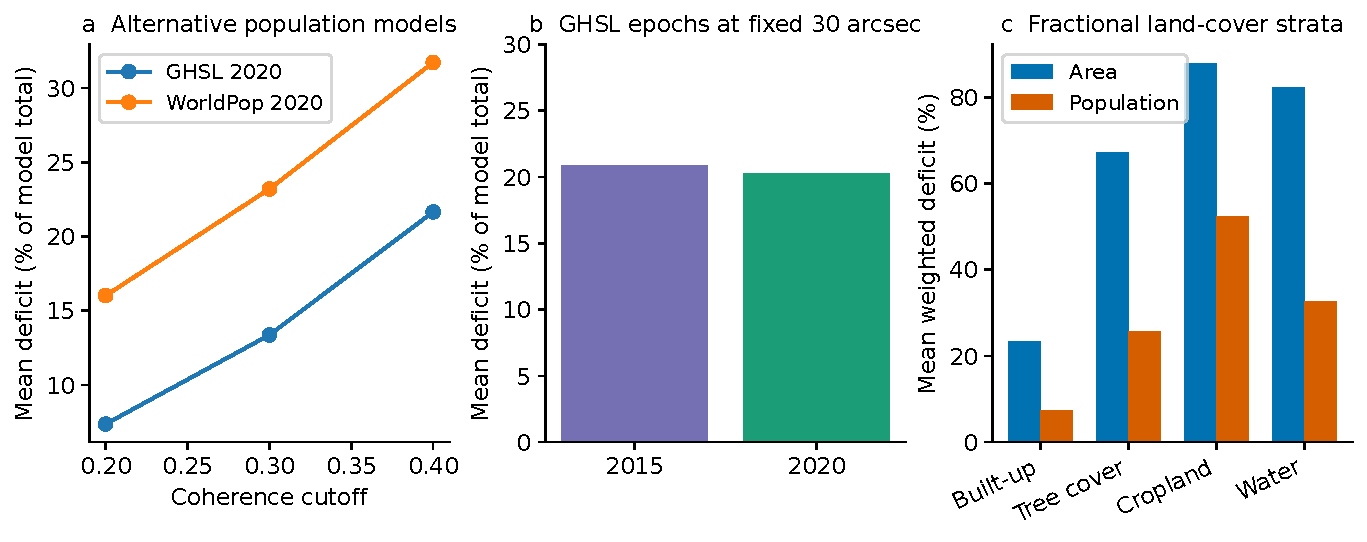
\includegraphics[width=\linewidth]{figures/F5_population_models.pdf}
\refstepcounter{figure}\label{fig:population}
\end{figure}


% begin cross_results.tex
\paragraph{Crossing population model and pair selection.} On the fixed GHSL--WorldPop common domain, both models are normalized to 22.358 million population units. At 1 km, uniform allocation exceeds the native-model deficit by 55.38--55.64\% for GHSL with the legacy 28 pairs and 51.29--51.51\% with the expanded 224 pairs. The corresponding WorldPop differences are 9.03--9.07\% and 8.64--8.68\%. All 16 model--sample--origin combinations have positive differences; normalized by the common total, these span 7.40--7.53 percentage points for GHSL and 2.09--2.13 for WorldPop. The direction therefore persists across these inputs, while its magnitude is strongly population-model dependent. The original approximately 58\% difference is specific to its full-domain GHSL case. Changing 28 to 224 pairs changes selection and composition as well as sample size; the comparison is not an isolated sample-size effect. Supplementary S12 reports every origin and the numerical convergence check.

% end cross_results.tex


\subsection{Matched processing and transfer to actual published support}

% begin matched_results.tex
Full-stack quality rejection leaves 431 of 437 pairs for inversion; the training branch retains 382 of 393 inputs. The full quality mask accepts 97.02\% of pixels and 99.71\% of the small area's allocated population. Among pixels with matched-input mean support below 0.2, 83.34\% still pass the fixed multi-index mask; the 0.8--1 group has 99.72\% acceptance. Low coherence-screened support is therefore not equivalent to final processing rejection (Fig.~\ref{fig:matched}). Neither acceptance nor rejection is independent physical truth.

At a legacy-support threshold of 0.5, the low-support/accepted and high-support/rejected categories contain 208,609 and 30,637 population allocation units, respectively. That legacy comparison also changes the acquisition period and sample. The matched-input bins provide the within-period comparison: median bootstrap velocity spread is 1.343 versus 1.185 mm yr$^{-1}$ and median inversion residual is 0.673 versus 0.368 mm for the lowest and highest support groups. These associations describe quality differences rather than a binary validity surrogate.

Of 44 excluded pair edges, 44 meet the recorded prediction/reference conditions. Pooled held-out LOS displacement RMSE is 0.984 mm across evaluable observations. Training-mask accepted and rejected locations give 0.699 and 5.150 mm, respectively; the lowest and highest training-support bins give 2.338 and 0.412 mm. On common evaluable observations, time-series differences, training linear velocity and a zero-displacement baseline give 0.984, 11.751 and 11.784 mm. This edge holdout reconstructs pairs between dates already represented in training; shared date-dependent atmospheric phase can also be reconstructed. These are residuals against excluded interferograms with shared acquisitions, not out-of-time forecasts or external velocity accuracies or evidence about permanently missing motion. Exclusions and per-pair results are retained in Supplementary S7.

We additionally compare the same GHSL population field against two distinct support summaries on this processing grid: mean support across the 437 full-stack input pairs and the final LiCSBAS full-stack quality mask. Direct intersections between the native source cells and 1-km UTM cells show that uniform-area allocation increases the mean deficit by 3.066--3.189 percentage points of the fixed AOI population for the 437-pair support field, but by 0.108--0.117 points for the final quality mask across four grid origins. Their native deficits are 3.4539\% and 0.2944\%, respectively. These support definitions carry different processing information; their contrast is not an error comparison, and neither identifies deformation in invalid pixels. The source-to-grid intersections and numerical checks are reported in Supplementary S13.

We also imposed known masks on actual fitted LOS velocities, but only among pixels already accepted by the final quality mask. For a predeclared $-5$ mm yr$^{-1}$ LOS class, 30\% artificial removal and nominal 1.11-km cells, local observed-population prevalence had mean relative bias of +1.1\% under random removal, +5.2\% under clustered removal, $-30.1\%$ when high-spread pixels were preferentially removed, and +79.1\% when low-spread pixels were removed. Nearest-center sampling was much more biased under random removal (+99.7\%). These conditional errors use known velocities in artificially masked valid pixels and do not estimate motion in the original invalid area (Supplementary S14).


\begin{figure}[htbp]\centering
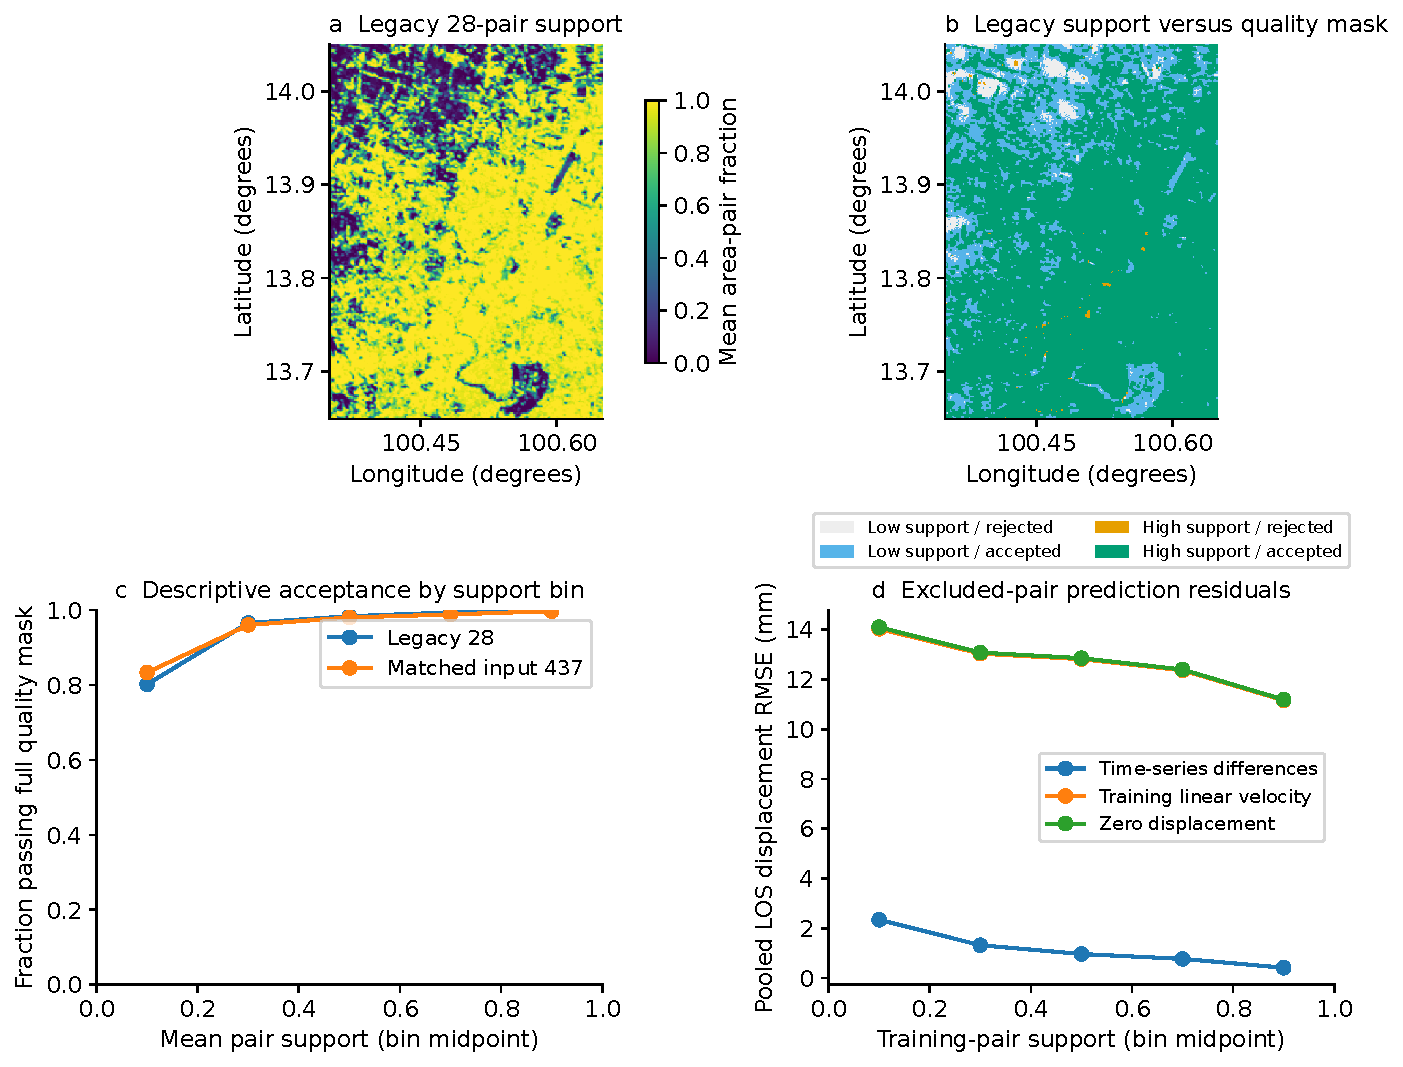
\includegraphics[width=\linewidth]{figures/F7_matched_processing.pdf}
\refstepcounter{figure}\label{fig:matched}
\end{figure}

% end matched_results.tex


In Fresno, the union of DWR observation cells covers 78.49\% of the 495.51-km$^2$ AOI but contains \DWRSupportPct{}\% of its allocated GHSL population. Of \DWRTotal{} population units, \DWRUnsupported{} fall outside the published footprint under the native allocation model. At 1 km, uniform allocation gives \DWRUniformMin{}--\DWRUniformMax{} units outside support. This is a substantial multiplier of a small baseline, but only about 1.2--1.3 percentage points of the AOI population in additional error. Both denominators matter. The larger origin sensitivity of center sampling illustrates a separate grid-placement vulnerability (Fig.~\ref{fig:dwr}). These are observations about coverage geometry and population allocation, not evidence of subsidence in the gaps. Using actual 2020 Census block geometries over the same complete-block domain, the Census-population-weighted mean DWR area-coverage fraction is 99.19\%, compared with 99.74\% under the native GHSL allocation; assigning whole Census block counts to blocks with at least 50\% observed area gives 99.41\%. These are cross-scale support statistics, not velocity classes, and the Census totals differ from GHSL (Supplementary S16). We additionally applied a published median-rate block classification to separate DWR/TRE ALTAMIRA vertical-rate rasters. For the 2015--2021 median of six annual products, valid rates cover blocks containing 95.70\% of complete-block Census population; 65.23\% of that covered population is assigned to blocks with median rates below $-5$ mm yr$^{-1}$. This is a transfer analysis using an interpolated vertical-rate product, not the manuscript's LOS field or an independent validation; annual and cumulative rate estimands yield materially different classes (Supplementary S17). A matched-domain comparison of GHSL and WorldPop 1-km allocations with Census block totals shows that both outperform an area-only allocation baseline, while normalized block-level WAPE remains 57--59\%; this coarse agreement test does not validate within-block population locations (Supplementary S19). A matched 100-m comparison that normalizes GHSL and CA-POP to identical Census block counts changes the outside-footprint allocation by 0.143 percentage points of the common Census total, with mixed tract-level directions; CA-POP uses those same block counts as source data (Supplementary S20). At the coarser 2020 block-group scale, the ACS 2017--2021 survey estimate totals 493,571; Census P1 is 0.36\% lower, while GHSL and WorldPop totals are 10.57\% and 6.03\% higher. This is a survey-based block-group agreement benchmark with unresolved source independence. It does not establish household locations or validate LOS deformation (Supplementary S24).

\begin{figure}[htbp]\centering
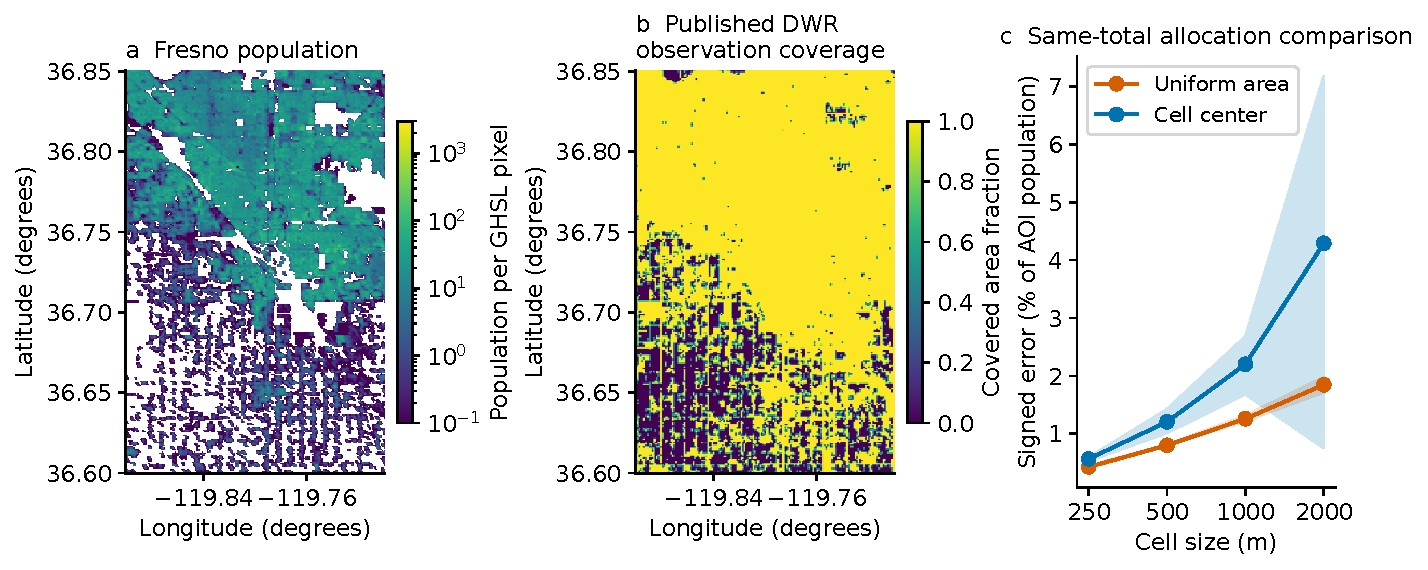
\includegraphics[width=\linewidth]{figures/F6_dwr.pdf}
\refstepcounter{figure}\label{fig:dwr}
\end{figure}

\FloatBarrier

% begin additional_results.tex
\subsection{Further stress tests and external transfer}
Actual irregular blocks expose an availability problem hidden by conditional error. At 30\% removal, native prevalence leaves 0.20\% of allocation unestimated under random pixels, versus 23.01\% under one hole and 28.64\% under four holes. The median rule leaves 9.41, 26.80 and 32.61\%, respectively. Native prevalence has smaller mean local L1 error at $-5$ mm yr$^{-1}$ on common-computable blocks, but whole-domain bound widths average 30.02, 24.02 and 30.97 pp. Small conditional errors do not identify class allocation under contiguous gaps (S25).

Spatially held-out recalibration gives GHSL WAPE 33.24--33.85\% versus 33.16\% in sample, and WorldPop 32.34--32.98\% versus 32.29\%. Local disagreement remains. Deleting each shared acquisition date changes the $q=0.3$ equal-quarter population deficit by $-0.386$ to $+0.165$ pp; these are dependent support sensitivities, not velocity re-inversions or confidence intervals (S26).

Raising training coherence from 0.2 to 0.4 reduces accepted population allocation from 99.40 to 95.34\% while pooled excluded-edge displacement RMSE falls from 0.491 to 0.388 mm; population-weighted RMSE changes from 0.344 to 0.336 mm. At 0.7, only 41.04\% of allocation remains. All 18 rules are retained, including nonmonotonic error under other metrics. These are post-filters on a fixed inversion, not absolute velocity accuracy (S27).

Across 96 fixed-region scale/origin/cutoff designs, uniform-minus-native differences are only 0.026--0.186 pp in Los Angeles and 0.051--0.372 pp in Davis--Sacramento. The direction transfers, but these small effects do not generalize the approximately 58\% primary-case relative difference (S28).

Strict municipal residential eligibility contains 85.22\% of mapped GHSL allocation and 89.30\% of mapped CA-POP allocation; 32.22 and 31.26\% of complete allocation lack mapped classification. Restricting weights to eligibility changes common-domain deficits from 0.0927/0.0572\% to 0.0508/0.0414\%. The joint domain covers only 89.13\% of complete Census population, failing the initial 90\% diagnostic gate. This is limited-domain sensitivity, not household-placement validation (S29).

External GNSS consistency is mixed. Native-pixel RMSE in Los Angeles is 14.49 mm yr$^{-1}$ under provider reference P597 and 1.30 under location-selected local control MHMS (11 validation stations). Davis--Sacramento gives 8.94 under P266 and 10.85 under UCD1 (four stations). All controls are excluded from validation; all sampling-radius outcomes remain. Archived source-version conflicts, different temporal models and dependent stations prevent uniform physical-validation claims or transfer to our Bangkok inversion (S30).

% end additional_results.tex


\section{Discussion}
\subsection{The aggregation effect and its dependence on inputs}
The matched-input comparisons establish a material change in population-weighted support summaries when fine spatial allocation is replaced by uniform coarse allocation. The effect persists in complete interior cells, so boundary handling does not explain the primary result. Crossing population models and pair selections gives a consistent positive direction across the 16 tested cases, but the relative difference is much smaller with WorldPop than with GHSL. This distinction matters: the approximately 58\% primary-case result demonstrates a consequential aggregation effect, while the crossed experiment measures how its magnitude depends on the selected population distribution. It does not establish a universal correction factor.

\subsection{Mechanism and choice of allocation method}
The mechanism is the loss of the population--support cross moment when a coarse mean support is multiplied by a coarse population total. Its signed effect follows within-cell covariance, explaining both the primary aggregate overestimation and the opposite directions under density-associated masking. Small aggregate biases under density-independent masks also identify conditions in which uniform allocation can be adequate. A finer overlay is useful when the selected population model's spatial structure is appropriate to retain; agreement with that reference does not establish household-level accuracy.

Method choice follows the available information. A complete-case overlay describes allocation inside its observed domain. A center rule is inexpensive but can miss subcell structure and boundary coverage. Uniform-area transfer is appropriate when its uniformity approximation produces acceptably small error for the intended summary. Building weights add ancillary assumptions and can share inputs with the population model. Imputation, multiple sensors and ground measurements add information about deformation and require their own evaluation. Our experiments quantify the effects of support accounting choices that accompany such measurements.

\subsection{Applicability and evidence limits}
The principal Chao Phraya statistic averages over area and selected interferometric pairs. It cannot identify how many unique residents lacked all observations, nor whether a final product is valid at their locations. A coherence pass is insufficient for a reliable velocity, and a failed pass does not prove permanent radar blindness. The matched processing experiment adds evidence about one specified processing chain: sampled support and its final quality mask are distinct, while held-out edge residuals assess internal reconstruction. Shared acquisition dates and atmospheric signals limit the physical interpretation of those residuals.

The crossed comparison and separate common-coverage population summaries both show that population-model choice is consequential. Local census geography, building occupancy and rapidly changing settlements are not measured by this overlay. The primary domains, added California rectangles and deliberate sampling designs do not establish a worldwide error magnitude. The primary domain inherits the finite source-VLM footprint; conclusions do not extend to locations outside it. LiCSAR's sampled pair support and DWR's published observation footprint remain different support objects, even though the same mass-preserving accounting protocol can be applied to both.

\paragraph{What the additional evidence supports.} Controlled masks and geometry/conservation checks evaluate numerical accounting against declared references. LiCSBAS excluded-edge residuals evaluate internal reconstruction, while the published DWR footprint and rate examples test transfer across product definitions. Census/CA-POP comparisons assess population-model allocation at reporting-unit scale, and ACS supplies a survey-based aggregate agreement benchmark with replicate-based uncertainty. These sources do not establish household locations or deformation in permanently unsupported pixels. The added California comparison supplies archived independent GNSS observations for an external LOS product, with mixed results and a temporal-model limitation; it does not validate our Bangkok inversion. No matched independent GNSS or leveling validation has been obtained for that inversion.


% begin additional_discussion.tex
\paragraph{Limits revealed by the added tests.} Small conditional error can coexist with large unestimated allocation, and stricter filters can reduce residuals by discarding coverage. Spatial recalibration does not remove population disagreement; small regional effects limit transfer of the primary magnitude. Municipal eligibility has incomplete coverage and a different vintage. Mixed California GNSS consistency supplies independent observations on an external product, with disjoint controls and temporal-model limits, but does not validate Bangkok, household placement or missing deformation. Availability and sensitivity should accompany any reported allocation effect.

% end additional_discussion.tex


\paragraph{Earlier estimates and source attribution.} The submitted 3.772492-million center-majority total is reproducible, but it is not a verified count of people exposed to subsidence in missing areas. The revised mean support-deficit estimand and its references are stated explicitly. Supplementary S2 retains the factorial lineage audit and conflicting archive branches. We have removed the exploratory Iran branch from quantitative applications. Its archived rate and mask correspond to the 2014--2020 product associated with Haghshenas Haghighi and Motagh (2024). No Iran result or new/old Iranian product comparison contributes to the quantitative conclusions. Supplementary S8 documents the attribution correction and distinguishes the newer products of Payne et al.\ \citep{haghshenas2024iran,payne2025iran,payne2024data}.

\section{Conclusions}
Spatial aggregation materially changes population-weighted InSAR support summaries by omitting the within-cell population--support cross moment. The same-input and complete-interior comparisons establish this effect; controlled missingness explains when its direction reverses or aggregate bias is small. Crossing population models with pair selections preserves the positive direction in the tested cases while showing strong variation in magnitude. Published observation polygons and two further California regions demonstrate transfer across support definitions while showing that the magnitude is case dependent. Actual irregular blocks, dependence checks, quality curves and municipal eligibility identify additional coverage and allocation limits; the external GNSS comparison yields mixed physical consistency. A useful reporting protocol therefore specifies its geographic denominator and support field, preserves extensive quantities and their cross moments, and reports allocation, population-model and sampling sensitivity. These results support transparent population-weighted accounting while keeping missing deformation an unresolved physical quantity.

\section*{Data Availability}
Public input data are obtained from COMET LiCSAR, GHSL, WorldPop, ESA WorldCover, the U.S. Census Bureau, California DWR, the archived ARIA California products, NGL and City of Fresno municipal GIS. Exact source-product identifiers, acquisition methods and input checksums are documented in the Supplementary Information and accompanying reproducibility materials. Source-provider terms govern access to and reuse of third-party inputs. Frozen processed analysis inputs, full reference and replicate tables, figure source data and the manuscript number ledger are publicly available with the versioned scientific reproduction package.

\section*{Code Availability}
The scientific reproduction package is publicly available at the fixed GitHub release \href{https://github.com/niubisile-wq/openinsar-observability-bias/releases/tag/v0.5.0}{v0.5.0}, commit \path{f70124f1cdc11e43848ce97c01f49fad6f7efb62}. It contains the experiment code, configurations, input manifests and checksums, processed analysis inputs, full reference outputs, environment records and reviewer reproduction instructions. Companion assets supply portable inputs and selected complete source products for S25--S30, with file-level checksums. The complete ACS files and official Census source archives used in S20 remain available at v0.4.1. All six new experiments are numerically rerun and compared with their full reference tables. Other provider-controlled original products and the complete interferogram processing stacks are obtained separately through the documented acquisition routes. The earlier DOI \href{https://doi.org/10.5281/zenodo.21444768}{10.5281/zenodo.21444768} archives v0.3.0; a revised DOI deposit remains pending.
\def\bibfont{\small}
\begin{thebibliography}{10}
\expandafter\ifx\csname url\endcsname\relax
  \def\url#1{\burl{#1}}\fi
\expandafter\ifx\csname urlprefix\endcsname\relax\def\urlprefix{URL }\fi
\providecommand{\bibinfo}[2]{#2}
\providecommand{\eprint}[2][]{\url{#2}}
\providecommand{\doi}[1]{\url{https://doi.org/#1}}
\bibcommenthead

\bibitem{ferretti2001ps}
\bibinfo{author}{Ferretti, A.}, \bibinfo{author}{Prati, C.} \&
  \bibinfo{author}{Rocca, F.}
\newblock \bibinfo{title}{Permanent scatterers in {SAR} interferometry}.
\newblock \emph{\bibinfo{journal}{IEEE Transactions on Geoscience and Remote
  Sensing}} \textbf{\bibinfo{volume}{39}}, \bibinfo{pages}{8--21}
  (\bibinfo{year}{2001}).

\bibitem{berardino2002sbas}
\bibinfo{author}{Berardino, P.}, \bibinfo{author}{Fornaro, G.},
  \bibinfo{author}{Lanari, R.} \& \bibinfo{author}{Sansosti, E.}
\newblock \bibinfo{title}{A new algorithm for surface deformation monitoring
  based on small baseline differential {SAR} interferograms}.
\newblock \emph{\bibinfo{journal}{IEEE Transactions on Geoscience and Remote
  Sensing}} \textbf{\bibinfo{volume}{40}}, \bibinfo{pages}{2375--2383}
  (\bibinfo{year}{2002}).

\bibitem{ferretti2011squeeSAR}
\bibinfo{author}{Ferretti, A.} \emph{et~al.}
\newblock \bibinfo{title}{A new algorithm for processing interferometric
  data-stacks: {SqueeSAR}}.
\newblock \emph{\bibinfo{journal}{IEEE Transactions on Geoscience and Remote
  Sensing}} \textbf{\bibinfo{volume}{49}}, \bibinfo{pages}{3460--3470}
  (\bibinfo{year}{2011}).

\bibitem{morishita2020licsbas}
\bibinfo{author}{Morishita, Y.} \emph{et~al.}
\newblock \bibinfo{title}{{LiCSBAS}: An open-source {InSAR} time series
  analysis package integrated with the {LiCSAR} automated {Sentinel-1} {InSAR}
  processor}.
\newblock \emph{\bibinfo{journal}{Remote Sensing}}
  \textbf{\bibinfo{volume}{12}}, \bibinfo{pages}{424} (\bibinfo{year}{2020}).

\bibitem{yunjun2019mintpy}
\bibinfo{author}{Zhang, Y.}, \bibinfo{author}{Fattahi, H.} \&
  \bibinfo{author}{Amelung, F.}
\newblock \bibinfo{title}{Small baseline {InSAR} time series analysis:
  Unwrapping error correction and noise reduction}.
\newblock \emph{\bibinfo{journal}{Computers \& Geosciences}}
  \textbf{\bibinfo{volume}{133}}, \bibinfo{pages}{104331}
  (\bibinfo{year}{2019}).

\bibitem{blackwell2020california}
\bibinfo{author}{Blackwell, E.}, \bibinfo{author}{Shirzaei, M.},
  \bibinfo{author}{Ojha, C.} \& \bibinfo{author}{Werth, S.}
\newblock \bibinfo{title}{Tracking california's sinking coast from space:
  Implications for relative sea-level rise}.
\newblock \emph{\bibinfo{journal}{Science Advances}}
  \textbf{\bibinfo{volume}{6}}, \bibinfo{pages}{eaba4551}
  (\bibinfo{year}{2020}).

\bibitem{fernandeztorres2024mexico}
\bibinfo{author}{Fernandez-Torres, E.~A.} \emph{et~al.}
\newblock \bibinfo{title}{Country-scale assessment of urban areas, population,
  and households exposed to land subsidence using sentinel-1 insar, and gps
  time series}.
\newblock \emph{\bibinfo{journal}{Natural Hazards}}
  \textbf{\bibinfo{volume}{120}}, \bibinfo{pages}{1577--1601}
  (\bibinfo{year}{2024}).

\bibitem{ao2024national}
\bibinfo{author}{Ao, Z.}, \bibinfo{author}{Hu, X.}, \bibinfo{author}{Tao, S.},
  \bibinfo{author}{Hu, X.} \emph{et~al.}
\newblock \bibinfo{title}{A national-scale assessment of land subsidence in
  china's major cities}.
\newblock \emph{\bibinfo{journal}{Science}}  (\bibinfo{year}{2024}).

\bibitem{ohenhen2025uscities}
\bibinfo{author}{Ohenhen, L.~O.}, \bibinfo{author}{Zhai, G.},
  \bibinfo{author}{Lucy, J.} \emph{et~al.}
\newblock \bibinfo{title}{Land subsidence risk to infrastructure in {US}
  metropolises}.
\newblock \emph{\bibinfo{journal}{Nature Cities}} \textbf{\bibinfo{volume}{2}},
  \bibinfo{pages}{543--554} (\bibinfo{year}{2025}).

\bibitem{xiong2026nationwide}
\bibinfo{author}{Xiong, Z.} \emph{et~al.}
\newblock \bibinfo{title}{Nationwide mapping and characterization of land
  subsidence in the {United States} using {InSAR}}.
\newblock \emph{\bibinfo{journal}{Remote Sensing of Environment}}
  \textbf{\bibinfo{volume}{333}}, \bibinfo{pages}{115134}
  (\bibinfo{year}{2026}).

\bibitem{yang2026buildingrisk}
\bibinfo{author}{Yang, M.}, \bibinfo{author}{Huang, W.}, \bibinfo{author}{Li,
  M.} \& \bibinfo{author}{Chang, L.}
\newblock \bibinfo{title}{From {PS-InSAR} observations to building-level risk:
  A data-driven framework for urban structural resilience}.
\newblock \emph{\bibinfo{journal}{Remote Sensing of Environment}}
  \textbf{\bibinfo{volume}{341}}, \bibinfo{pages}{115454}
  (\bibinfo{year}{2026}).

\bibitem{oelsmann2026coastal}
\bibinfo{author}{Oelsmann, J.}, \bibinfo{author}{Nicholls, R.~J.},
  \bibinfo{author}{Lincke, D.} \emph{et~al.}
\newblock \bibinfo{title}{Subsidence more than doubles sea-level rise today
  along densely populated coasts}.
\newblock \emph{\bibinfo{journal}{Nature Communications}}
  \textbf{\bibinfo{volume}{17}}, \bibinfo{pages}{4382} (\bibinfo{year}{2026}).

\bibitem{murray2025hawaii}
\bibinfo{author}{Murray, K.}, \bibinfo{author}{Barbee, M.},
  \bibinfo{author}{Thompson, P.} \& \bibinfo{author}{Fletcher, C.}
\newblock \bibinfo{title}{Coastal land subsidence accelerates timelines for
  future flood exposure in hawai'i}.
\newblock \emph{\bibinfo{journal}{Communications Earth \& Environment}}
  \textbf{\bibinfo{volume}{6}}, \bibinfo{pages}{123} (\bibinfo{year}{2025}).

\bibitem{luachapichatikul2020bangkok}
\bibinfo{author}{Luachapichatikul, S.}
\newblock \emph{\bibinfo{title}{Measuring Land Subsidence with {PS-InSAR} in
  {Bangkok} using {Sentinel-1} Time-Series Techniques}}.
\newblock \bibinfo{type}{Master's thesis}, \bibinfo{school}{Burapha University}
  (\bibinfo{year}{2020}).
\newblock \urlprefix\url{https://ir.buu.ac.th/dspace/handle/1513/311}.

\bibitem{pumpuang2024bangkapi}
\bibinfo{author}{Pumpuang, A.} \& \bibinfo{author}{Aobpaet, A.}
\newblock \bibinfo{title}{Evolution pattern of land subsidence using {InSAR}
  time-series analysis in {Bangkapi}, {Bangkok}, {Thailand}}.
\newblock \emph{\bibinfo{journal}{Journal of Current Science and Technology}}
  \textbf{\bibinfo{volume}{14}}, \bibinfo{pages}{49} (\bibinfo{year}{2024}).
\newblock
  \urlprefix\url{https://ph04.tci-thaijo.org/index.php/JCST/article/view/2549}.

\bibitem{aieorattanawadee2022bangkok}
\bibinfo{author}{Aieorattanawadee, N.}
\newblock \emph{\bibinfo{title}{Monitoring land subsidence in {Bangkok} during
  2018--2022 using time-series {InSAR} analysis with {MintPy}}}.
\newblock \bibinfo{type}{Master's thesis}, \bibinfo{school}{Chulalongkorn
  University} (\bibinfo{year}{2022}).
\newblock \urlprefix\url{https://digital.car.chula.ac.th/chulaetd/6585/}.

\bibitem{eicher2001dasymetric}
\bibinfo{author}{Eicher, C.~L.} \& \bibinfo{author}{Brewer, C.~A.}
\newblock \bibinfo{title}{Dasymetric mapping and areal interpolation:
  Implementation and evaluation}.
\newblock \emph{\bibinfo{journal}{Cartography and Geographic Information
  Science}} \textbf{\bibinfo{volume}{28}}, \bibinfo{pages}{125--138}
  (\bibinfo{year}{2001}).

\bibitem{mennis2003population}
\bibinfo{author}{Mennis, J.}
\newblock \bibinfo{title}{Generating surface models of population using
  dasymetric mapping}.
\newblock \emph{\bibinfo{journal}{The Professional Geographer}}
  \textbf{\bibinfo{volume}{55}}, \bibinfo{pages}{31--42}
  (\bibinfo{year}{2003}).

\bibitem{ohenhen2026deltas}
\bibinfo{author}{Ohenhen, L.~O.} \emph{et~al.}
\newblock \bibinfo{title}{Global subsidence of river deltas}.
\newblock \emph{\bibinfo{journal}{Nature}} \textbf{\bibinfo{volume}{649}},
  \bibinfo{pages}{894--901} (\bibinfo{year}{2026}).

\bibitem{ohenhen2025deltadata}
\bibinfo{author}{Ohenhen, L.}
\newblock \bibinfo{title}{Global subsidence of river deltas}
  (\bibinfo{year}{2025}).
\newblock \bibinfo{note}{1-km vertical land motion GeoTIFFs for 40 river
  deltas}.

\bibitem{licsarproducts}
\bibinfo{author}{{COMET}}.
\newblock \bibinfo{title}{{LiCSAR} product details} (\bibinfo{year}{2026}).
\newblock
  \urlprefix\url{https://comet.nerc.ac.uk/comet-lics-portal-product-details/}.
\newblock \bibinfo{note}{Accessed 27 September 2026; product-specific coherence
  encoding and unwrapped validity}.

\bibitem{pesaresi2024ghsl}
\bibinfo{author}{Pesaresi, M.} \emph{et~al.}
\newblock \bibinfo{title}{Advances on the global human settlement layer by
  joint assessment of earth observation and population survey data}.
\newblock \emph{\bibinfo{journal}{International Journal of Digital Earth}}
  \textbf{\bibinfo{volume}{17}}, \bibinfo{pages}{2390454}
  (\bibinfo{year}{2024}).

\bibitem{worldpop2020}
\bibinfo{author}{{WorldPop}}.
\newblock \bibinfo{title}{Thailand 2020 population counts: unconstrained,
  un-adjusted, 3 arc-second product} (\bibinfo{year}{2020}).
\newblock \urlprefix\url{https://hub.worldpop.org/geodata/summary?id=29165}.
\newblock \bibinfo{note}{File tha\_ppp\_2020\_UNadj.tif; accessed 27 September
  2026}.

\bibitem{worldcover2021}
\bibinfo{author}{Zanaga, D.}, \bibinfo{author}{Van De~Kerchove, R.},
  \bibinfo{author}{Daems, D.} \emph{et~al.}
\newblock \bibinfo{title}{{ESA WorldCover} 10 m 2021 v200}
  (\bibinfo{year}{2022}).

\bibitem{licsbas2}
\bibinfo{author}{Morishita, Y.}
\newblock \bibinfo{title}{{LiCSBAS2}: time-series processing software}
  (\bibinfo{year}{2026}).
\newblock \urlprefix\url{https://github.com/yumorishita/LiCSBAS2}.
\newblock \bibinfo{note}{Commit 2627e50a1c703becd4a0b18754b05c1cf8c564d5; local
  Windows I/O portability patch documented}.

\bibitem{dwr2026}
\bibinfo{author}{{California Department of Water Resources}}.
\newblock \bibinfo{title}{Vertical displacement point data locations, 2026q1:
  published observation-cell polygons} (\bibinfo{year}{2026}).
\newblock
  \urlprefix\url{https://gis.water.ca.gov/arcgis/rest/services/Elevation/Vertical_Displacement_Point_Data_Locations_2026Q1/MapServer}.
\newblock \bibinfo{note}{Service layer 0, geometry type polygon; accessed 27
  September 2026}.

\bibitem{dwrdocumentation}
\bibinfo{author}{{California Department of Water Resources}}.
\newblock \bibinfo{title}{{SGMA} data viewer documentation: {TRE Altamira
  InSAR} dataset} (\bibinfo{year}{2026}).
\newblock
  \urlprefix\url{https://sgma.water.ca.gov/webgis/config/custom/html/SGMADataViewer/doc/}.
\newblock \bibinfo{note}{100 m measurement support distinguished from
  interpolated display rasters; accessed 27 September 2026}.

\bibitem{sangha2026california}
\bibinfo{author}{Sangha, S.~S.}, \bibinfo{author}{Funning, G.~J.},
  \bibinfo{author}{Govorcin, M.} \& \bibinfo{author}{Bekaert, D. P.~S.}
\newblock \bibinfo{title}{A statewide insar velocity map for california
  produced by a comprehensive large scale analysis of aria standard products}.
\newblock \emph{\bibinfo{journal}{Earth and Space Science}}
  \textbf{\bibinfo{volume}{13}}, \bibinfo{pages}{e2026EA005214}
  (\bibinfo{year}{2026}).

\bibitem{sangha2026data}
\bibinfo{author}{Sangha, S.}, \bibinfo{author}{Funning, G.},
  \bibinfo{author}{Govorcin, M.} \& \bibinfo{author}{Bekaert, D.}
\newblock \bibinfo{title}{Data and software for sangha et al., 2026: A
  statewide insar velocity map for california} (\bibinfo{year}{2026}).
\newblock \bibinfo{note}{Fixed April 2026 archived version; CC BY 4.0}.

\bibitem{fresno2026landuse}
\bibinfo{author}{{City of Fresno}}.
\newblock \bibinfo{title}{Public existing land use gis layer}
  (\bibinfo{year}{2026}).
\newblock
  \urlprefix\url{https://services2.arcgis.com/WkBUojyNPhsWOk1W/arcgis/rest/services/Existing_Land_Use/FeatureServer/19}.
\newblock \bibinfo{note}{Hosted FeatureServer layer 19; ObjectID, ELU, ELUText
  and LayerRefreshDate; accessed 1 October 2026}.

\bibitem{haghshenas2024iran}
\bibinfo{author}{Haghshenas~Haghighi, M.} \& \bibinfo{author}{Motagh, M.}
\newblock \bibinfo{title}{Uncovering the impacts of depleting aquifers: A
  remote sensing analysis of land subsidence in iran}.
\newblock \emph{\bibinfo{journal}{Science Advances}}
  \textbf{\bibinfo{volume}{10}} (\bibinfo{year}{2024}).

\bibitem{payne2025iran}
\bibinfo{author}{Payne, J.~A.} \emph{et~al.}
\newblock \bibinfo{title}{Widespread extent of irrecoverable aquifer depletion
  revealed by country-wide analysis of land surface subsidence hazard in iran}.
\newblock \emph{\bibinfo{journal}{Journal of Geophysical Research: Solid
  Earth}} \textbf{\bibinfo{volume}{130}} (\bibinfo{year}{2025}).

\bibitem{payne2024data}
\bibinfo{author}{Payne, J.}
\newblock \bibinfo{title}{Accompanying data for paper: Widespread extent of
  irrecoverable aquifer depletion revealed by country-wide analysis of land
  surface subsidence hazard in iran} (\bibinfo{year}{2024}).

\end{thebibliography}

\section*{Author Contributions}
Z.L.: analysis and manuscript preparation. W.X.: supervision and manuscript revision.
\section*{Additional Information}
\subsection*{Competing interests}
The authors declare no competing interests.
\section*{Figure legends}


\noindent\textbf{Figure 1.} Fixed-footprint Chao Phraya analysis: GHSL 2020 population, mean joint area--pair support at $q=0.3$, and their allocation-weighted support deficit. Maps use the native GHSL grid; logarithmic population displays leave zero values blank. No panel maps verified hazard in unsupported locations.

\noindent\textbf{Figure 2.} Continuous support summaries. Left: weighted distributions of native-pixel mean support for $q=0.3$. Right: mean deficits under three coherence cutoffs. These curves use one frozen geographic domain and do not condition on an unverified velocity scale.

\noindent\textbf{Figure 3.} Same-input allocation comparisons at $q=0.3$. Lines are means across four origins and bands span those origins, not confidence intervals. Errors are normalized by fixed AOI exposure totals. The local 1-km plot shows uniform-minus-native error divided by each nonzero cell population; its negative values demonstrate that aggregate overestimation is not universal at the cell scale.

\noindent\textbf{Figure 4.} Artificial missingness in the fixed Bangkok rectangle, using 10-fine-pixel coarse cells and zero origin. Symbols show mean signed error and bars the 2.5th--97.5th percentiles of 100 introduced-mask repetitions. The denominator is the entire test-domain population, enabling comparison when the removed population is very small. Complete relative-error, local-error, scale and origin results are provided separately.

\noindent\textbf{Figure 5.} Population and land-cover sensitivities. Population models and epoch comparisons use their common valid domain; the epoch panel holds spatial resolution fixed. Fractional land-cover summaries use the primary geographic domain and preserve the within-GHSL-pixel allocation assumption. WorldCover 2021 v200: \copyright{} ESA WorldCover project 2021; contains modified Copernicus Sentinel data (2021) processed by the ESA WorldCover consortium.

\noindent\textbf{Figure 6.} Matched LiCSBAS experiment in the fixed Bangkok rectangle. The legacy support map uses the 2016--2022 sample; its high/low split is 0.5 in panel b, compared with the 2019--2020 full-stack quality mask. Panel c separately includes the matched 437-pair input diagnostic. Both diagnostics use coherence cutoff $q=0.3$. Panel d groups held-out prediction residuals using training pairs only. Bin connections guide the eye; no independent-observation confidence interval is implied

\noindent\textbf{Figure 7.} Second-region accounting using actual DWR observation-cell polygons in a fixed Fresno rectangle. Polygon intersections are unioned before assigning population. The deficit reference is small because the observed footprint covers almost all allocated population despite leaving appreciable area uncovered. Scale-comparison errors use the full AOI population as denominator; bands span four origins.

\section*{Table legends}
\noindent\textbf{Table 1.} Native-model support summaries for the geographic domain and legacy 28-pair sample. Population deficit is in million mean allocation units; built-surface deficit is in km$^2$. Percentages use the appropriate fixed exposure total.
\end{document}
